\documentclass[12pt, a4paper]{article}

\usepackage[T2A]{fontenc}
\usepackage[utf8]{inputenc}
\usepackage[main=russian, english]{babel}

\usepackage{microtype}
\sloppy


%% ГОСТ 7.32-2017
%% 6.1 Общие требования
%%
%% 6.1.1 Изложение текста и оформление отчёта выполняют в соответствии с требованиями настоящего стандарта.
%% Страницы текста отчёта о НИР и включённые в отчёт иллюстрации и таблицы должны соответствовать формату А4 по ГОСТ 9327.
%% Допускается применение формата А3 при наличии большого количества таблиц и иллюстраций данного формата.
%%
%% Отчёт о НИР должен быть выполнен любым печатным способом на одной стороне листа белой бумаги формата А4 через полтора интервала.

\usepackage[onehalfspacing]{setspace}

%% Допускается при подготовке заключительного отчёта о НИР печатать через один интервал, если отчёт имеет значительный объём (500 и более страниц).
%% Цвет шрифта должен быть чёрным, размер шрифта — не менее 12 пт.
%% Рекомендуемый тип шрифта для основного текста отчёта — Times New Roman.

%\usepackage{paratype}
%\renewcommand{\rmdefault}{PTSerif-TLF}
%\renewcommand{\ttdefault}{PTMono-TLF}

%% Полужирный шрифт применяют только для заголовков разделов и подразделов, заголовков структурных элементов.
%% Использование курсива допускается для обозначения объектов (биология, геология, медицина, нанотехнологии, генная инженерия и др.) и написания терминов (например, in vivo, in vitro) и иных объектов и терминов на латыни.
%%
%% Для акцентирования внимания может применяться выделение текста с помощью шрифта иного начертания, чем шрифт основного текста, но того же кегля и гарнитуры.
%% Разрешается для написания определённых терминов, формул, теорем применять шрифты разной гарнитуры.
%%
%% Текст отчёта следует печатать, соблюдая следующие размеры полей: левое — 30 мм, правое — 15 мм, верхнее и нижнее — 20 мм.

\newcommand{\PageLeftMargin}{30mm}
\newcommand{\PageRightMargin}{15mm}
\newcommand{\PageTopMargin}{20mm}
\newcommand{\PageBottomMargin}{20mm}

\usepackage[
	left=\PageLeftMargin,
	right=\PageRightMargin,
	top=\PageTopMargin,
	bottom=\PageBottomMargin,
]{geometry}

%% Абзацный отступ должен быть одинаковым по всему тексту отчёта и равен 1,25 см.

\usepackage{indentfirst}
\setlength{\parindent}{1.25cm}

\setlength{\parskip}{1ex}

%%
%% 6.1.2 Вне зависимости от способа выполнения отчёта качество напечатанного текста и оформления иллюстраций, таблиц, распечаток программ должно удовлетворять требованию их чёткого воспроизведения.
%%
%% 6.1.3 При выполнении отчёта о НИР необходимо соблюдать равномерную плотность и чёткость изображения по всему отчёту.
%% Все линии, буквы, цифры и знаки должны иметь одинаковую контрастность по всему тексту отчёта.
%%
%% 6.1.4 Фамилии, наименования учреждений, организаций, фирм, наименования изделий и другие имена собственные в отчёте приводят на языке оригинала.
%% Допускается транслитерировать имена собственные и приводить наименования организаций в переводе на язык отчёта с добавлением (при первом упоминании) оригинального названия по ГОСТ 7.79.
%%
%% 6.1.5 Сокращения слов и словосочетаний на русском, белорусском [1] и иностранных европейских языках оформляют в соответствии с требованиями ГОСТ 7.11, ГОСТ 7.12.
%%   [1] Для Республики Беларусь применим СТБ 7.12.
%%
%% 6.2 Построение отчёта
%%
%% 6.2.1 Наименования структурных элементов отчёта: "СПИСОК ИСПОЛНИТЕЛЕЙ", "РЕФЕРАТ", "СОДЕРЖАНИЕ", "ТЕРМИНЫ И ОПРЕДЕЛЕНИЯ", "ПЕРЕЧЕНЬ СОКРАЩЕНИЙ И ОБОЗНАЧЕНИЙ", "ВВЕДЕНИЕ", "ЗАКЛЮЧЕНИЕ", "СПИСОК ИСПОЛЬЗОВАННЫХ ИСТОЧНИКОВ", "ПРИЛОЖЕНИЕ" служат заголовками структурных элементов отчёта.

\AtBeginDocument{\renewcommand\contentsname{Содержание}}

%%
%% Заголовки структурных элементов следует располагать в середине строки без точки в конце, прописными буквами, не подчёркивая.
%% Каждый структурный элемент и каждый раздел основной части отчёта начинают с новой страницы.

\usepackage{titlesec}

\newcommand{\ChapterLeftMargin}{}
\newcommand{\ChapterFormat}{}
\newcommand{\ChapterSep}{}
\newcommand{\ChapterBeforeCode}{}

\newcommand{\SetMainPartChapterSettings}{%
	\renewcommand{\ChapterLeftMargin}{\parindent}%
	\renewcommand{\ChapterFormat}{\bfseries}%
	\renewcommand{\ChapterSep}{1em}%
	\renewcommand{\ChapterBeforeCode}{}%
}

\newcommand{\SetStructuralElementChapterSettings}{%
	\renewcommand{\ChapterLeftMargin}{0pt}%
	\renewcommand{\ChapterFormat}{\filcenter\bfseries}%
	\renewcommand{\ChapterSep}{}%
	\renewcommand{\ChapterBeforeCode}{\MakeUppercase}%
}

\SetStructuralElementChapterSettings

\titlespacing*{\chapter}{\ChapterLeftMargin}{-30pt}{8pt}
\titleformat{\chapter}[block]{\ChapterFormat}{\thechapter}{\ChapterSep}{\ChapterBeforeCode}{}

\newcommand{\StructuralElement}[1]{%
	\chapter*{#1}%
	\addcontentsline{toc}{chapter}{\MakeUppercase{#1}}%
}

\newenvironment{MainPart}%
	{\SetMainPartChapterSettings}%
	{\SetStructuralElementChapterSettings}

%%
%% 6.2.2 Основную часть отчёта следует делить на разделы, подразделы и пункты.
%% Пункты при необходимости могут делиться на подпункты.
%% Разделы и подразделы отчёта должны иметь заголовки.
%% Пункты и подпункты, как правило, заголовков не имеют.
%%
%% 6.2.3 Заголовки разделов и подразделов основной части отчёта следует начинать с абзацного отступа и размещать после порядкового номера, печатать с прописной буквы, полужирным шрифтом, не подчёркивать, без точки в конце.
%% Пункты и подпункты могут иметь только порядковый номер без заголовка, начинающийся с абзацного отступа.

\titlespacing*{\section}{\parindent}{*4}{*2}
\titlespacing*{\subsection}{\parindent}{*4}{*4}
\titlespacing*{\subsubsection}{\parindent}{*4}{*4}
\titlespacing*{\paragraph}{\parindent}{*0}{*1}
\titleformat{\section}{\bfseries}{\thesection}{1em}{}{}{}
\titleformat{\subsection}{\bfseries}{\thesubsection}{1em}{}{}{}
\titleformat{\subsubsection}{\bfseries}{\thesubsubsection}{1em}{}{}{}

%%
%% 6.2.4 Если заголовок включает несколько предложений, их разделяют точками.
%% Переносы слов в заголовках не допускаются.
%%
%% 6.3 Нумерация страниц отчёта
%%
%% 6.3.1 Страницы отчёта следует нумеровать арабскими цифрами, соблюдая сквозную нумерацию по всему тексту отчёта, включая приложения.
%% Номер страницы проставляется в центре нижней части страницы без точки.
%% Приложения, которые приведены в отчёте о НИР и имеющие собственную нумерацию, допускается не перенумеровать.
%%
%% 6.3.2 Титульный лист включают в общую нумерацию страниц отчёта.
%% Номер страницы на титульном листе не проставляют.
%%
%% 6.3.3 Иллюстрации и таблицы, расположенные на отдельных листах, включают в общую нумерацию страниц отчёта.
%% Иллюстрации и таблицы на листе формата А3 учитывают как одну страницу.
%%
%% 6.4 Нумерация разделов, подразделов, пунктов, подпунктов и книг отчёта
%%
%% 6.4.1 Разделы должны иметь порядковые номера в пределах всего отчёта, обозначенные арабскими цифрами без точки и расположенные с абзацного отступа.
%% Подразделы должны иметь нумерацию в пределах каждого раздела.
%% Номер подраздела состоит из номеров раздела и подраздела, разделённых точкой.
%% В конце номера подраздела точка не ставится.
%% Разделы, как и подразделы, могут состоять из одного или нескольких пунктов.
%%
%% 6.4.2 Если отчёт не имеет подразделов, то нумерация пунктов в нем должна быть в пределах каждого раздела и номер пункта должен состоять из номеров раздела и пункта, разделённых точкой.
%% В конце номера пункта точка не ставится.
%%
%% Если отчёт имеет подразделы, то нумерация пунктов должна быть в пределах подраздела и номер пункта должен состоять из номеров раздела, подраздела и пункта, разделённых точками.
%%
%% 6.4.3 Если раздел или подраздел состоит из одного пункта, то пункт не нумеруется.
%%
%% 6.4.4 Если текст отчёта подразделяется только на пункты, они нумеруются порядковыми номерами в пределах отчёта.
%%
%% 6.4.5 Пункты при необходимости могут быть разбиты на подпункты, которые должны иметь порядковую нумерацию в пределах каждого пункта: 4.2.1.1, 4.2.1.2, 4.2.1.3 и т.д.

\setcounter{tocdepth}{3}
\setcounter{secnumdepth}{3}

%%
%% 6.4.6 Внутри пунктов или подпунктов могут быть приведены перечисления.
%% Перед каждым элементом перечисления следует ставить тире.

\renewcommand{\labelitemi}{—}
\renewcommand{\labelitemii}{—}

%% При необходимости ссылки в тексте отчёта на один из элементов перечисления вместо тире ставят строчные буквы русского алфавита со скобкой, начиная с буквы "а" (за исключением букв ё, з, й, о, ч, ъ, ы, ь).

\renewcommand{\labelenumi}{\asbuk{enumi})}
\renewcommand{\labelenumii}{\arabic{enumii})}
\usepackage{enumitem}

\makeatletter
	\AddEnumerateCounter{\asbuk}{\@asbuk}{ю)}
\makeatother
\setlist{nosep, leftmargin=\parindent}

%% Простые перечисления отделяются запятой, сложные — точкой с запятой.
%%
%% При наличии конкретного числа перечислений допускается перед каждым элементом перечисления ставить арабские цифры, после которых ставится скобка.
%%
%% Перечисления приводятся с абзацного отступа в столбик.
%%
%% 6.4.7 Заголовки должны чётко и кратко отражать содержание разделов, подразделов.
%% Если заголовок состоит из двух предложений, их разделяют точкой.
%%
%% 6.4.8 Если отчёт состоит из двух и более книг, каждая книга должна иметь свой порядковый номер.
%% Номер каждой книги следует проставлять арабскими цифрами на титульном листе под указанием вида отчёта: "Книга 2".
%%
%% 6.5 Иллюстрации

\usepackage{graphicx}
\usepackage{float}

\usepackage[tableposition=top, singlelinecheck=false]{caption}
\usepackage{subcaption}

\DeclareCaptionLabelFormat{gostfigure}{Рисунок #2}
\DeclareCaptionLabelFormat{gosttable}{Таблица #2}
\DeclareCaptionLabelSeparator{gost}{~—~}
\captionsetup{labelsep=gost}
\captionsetup*[figure]{labelformat=gostfigure}
\captionsetup*[table]{labelformat=gosttable}
\renewcommand{\thesubfigure}{\asbuk{subfigure}}

\usepackage{multirow}
\usepackage[table,xcdraw]{xcolor}

%%
%% 6.5.1 Иллюстрации (чертежи, графики, схемы, компьютерные распечатки, диаграммы, фотоснимки) следует располагать в отчёте непосредственно после текста отчёта, где они упоминаются впервые, или на следующей странице (по возможности ближе к соответствующим частям текста отчёта).
%% На все иллюстрации в отчёте должны быть даны ссылки.
%% При ссылке необходимо писать слово "рисунок" и его номер, например: "в соответствии с рисунком 2" и т.д.

\newcommand{\imght}[3]{%
	\begin{figure}[ht]%
		\center{\includegraphics[#1]{inc/img/#2}}%
		\captionsetup{justification=centering}%
		\caption{#3}%
		\label{img:#2}%
	\end{figure}%
}

\newcommand{\imgH}[3]{%
	\begin{figure}[H]%
		\center{\includegraphics[#1]{inc/img/#2}}%
		\captionsetup{justification=centering}%
		\caption{#3}%
		\label{img:#2}%
	\end{figure}%
}

\usepackage{pgfplots}

%%
%% 6.5.2 Чертежи, графики, диаграммы, схемы, помещаемые в отчёте, должны соответствовать требованиям стандартов Единой системы конструкторской документации (ЕСКД).
%%
%% 6.5.3 Количество иллюстраций должно быть достаточным для пояснения излагаемого текста отчёта.
%% Не рекомендуется в отчёте о НИР приводить объёмные рисунки.
%%
%% 6.5.4 Иллюстрации, за исключением иллюстраций, приведённых в приложениях, следует нумеровать арабскими цифрами сквозной нумерацией.
%% Если рисунок один, то он обозначается: Рисунок 1.
%%   Пример — Рисунок 1 — Схема прибора
%%
%% 6.5.5 Иллюстрации каждого приложения обозначают отдельной нумерацией арабскими цифрами с добавлением перед цифрой обозначения приложения: Рисунок А.3.
%%
%% 6.5.6 Допускается нумеровать иллюстрации в пределах раздела отчёта.
%% В этом случае номер иллюстрации состоит из номера раздела и порядкового номера иллюстрации, разделённых точкой: Рисунок 2.1.
%%
%% 6.5.7 Иллюстрации при необходимости могут иметь наименование и пояснительные данные (подрисуночный текст).
%% Слово "Рисунок", его номер и через тире наименование помещают после пояснительных данных и располагают в центре под рисунком без точки в конце.
%%   Пример — Рисунок 2 — Оформление таблицы
%%
%% 6.5.8 Если наименование рисунка состоит из нескольких строк, то его следует записывать через один межстрочный интервал.
%% Наименование рисунка приводят с прописной буквы без точки в конце.
%% Перенос слов в наименовании графического материала не допускается.
%%
%% 6.6 Таблицы

\renewcommand{\arraystretch}{1.3}

\newcommand{\TableHeader}[2]{%
	\parbox{#1}{%
		\vspace{.5\baselineskip}%
		\centering{\textbf{#2}}%
		\vspace{.5\baselineskip}%
	}%
}

%%
%% 6.6.1 Цифровой материал должен оформляться в виде таблиц.
%% Таблицы применяют для наглядности и удобства сравнения показателей.
%%
%% 6.6.2 Таблицу следует располагать непосредственно после текста, в котором она упоминается впервые, или на следующей странице.
%%
%% На все таблицы в отчёте должны быть ссылки.
%% При ссылке следует печатать слово "таблица" с указанием её номера.
%%
%% 6.6.3 Наименование таблицы, при ее* наличии, должно отражать её содержание, быть точным, кратким.
%% Наименование следует помещать над таблицей слева, без абзацного отступа в следующем формате: Таблица Номер таблицы — Наименование таблицы.
%% Наименование таблицы приводят с прописной буквы без точки в конце.
%%   * Вероятно ошибка оригинала. Следует читать "его". - Примечание изготовителя базы данных.
%%
%% Если наименование таблицы занимает две строки и более, то его следует записывать через один межстрочный интервал.
%%
%% Таблицу с большим количеством строк допускается переносить на другую страницу.
%% При переносе части таблицы на другую страницу слово "Таблица", её номер и наименование указывают один раз слева над первой частью таблицы, а над другими частями также слева пишут слова "Продолжение таблицы" и указывают номер таблицы.
%%
%% При делении таблицы на части допускается её головку или боковик заменять соответственно номерами граф и строк.
%% При этом нумеруют арабскими цифрами графы и (или) строки первой части таблицы.
%% Таблица оформляется в соответствии с рисунком 1.
%%
%% 6.6.4 Таблицы, за исключением таблиц приложений, следует нумеровать арабскими цифрами сквозной нумерацией.
%%
%% Таблицы каждого приложения обозначаются отдельной нумерацией арабскими цифрами с добавлением перед цифрой обозначения приложения.
%% Если в отчёте одна таблица, она должна быть обозначена "Таблица 1" или "Таблица А.1" (если она приведена в приложении А).
%%
%% Допускается нумеровать таблицы в пределах раздела при большом объёме отчёта.
%% В этом случае номер таблицы состоит из номера раздела и порядкового номера таблицы, разделённых точкой: Таблица 2.3.
%%
%% 6.6.5 Заголовки граф и строк таблицы следует печатать с прописной буквы, а подзаголовки граф — со строчной буквы, если они составляют одно предложение с заголовком, или с прописной буквы, если они имеют самостоятельное значение.
%% В конце заголовков и подзаголовков таблиц точки не ставятся.
%% Названия заголовков и подзаголовков таблиц указывают в единственном числе.
%%
%% 6.6.6 Таблицы слева, справа, сверху и снизу ограничивают линиями.
%% Разделять заголовки и подзаголовки боковика и граф диагональными линиями не допускается.
%% Заголовки граф выравнивают по центру, а заголовки строк — по левому краю.
%%
%% Горизонтальные и вертикальные линии, разграничивающие строки таблицы, допускается не проводить, если их отсутствие не затрудняет пользование таблицей.
%%
%% 6.6.7 Текст, повторяющийся в строках одной и той же графы и состоящий из одиночных слов, заменяют кавычками.
%% Ставить кавычки вместо повторяющихся цифр, буквенно-цифровых обозначений, знаков и символов не допускается.
%%
%% Если текст повторяется, то при первом повторении его заменяют словами "то же", а далее кавычками.
%%
%% В таблице допускается применять размер шрифта меньше, чем в тексте отчёта.
%%
%% 6.7 Примечания и сноски

\renewcommand*{\thefootnote}{\arabic{footnote})}
\renewcommand{\footnoterule}{%
	\kern -3pt%
	\hrule width 40mm height .4pt%
	\kern 2.6pt%
}

%%
%% 6.7.1 Примечания приводят в отчёте, если необходимы пояснения или справочные данные к содержанию текста, таблиц или графического материала.
%%
%% 6.7.2 Слово "Примечание" следует печатать с прописной буквы с абзацного отступа, не подчёркивая.
%%
%% 6.7.3 Примечания следует помещать непосредственно после текстового, графического материала или таблицы, к которым относятся эти примечания.
%% Если примечание одно, то после слова "Примечание" ставится тире и текст примечания печатают с прописной буквы.
%% Одно примечание не нумеруется. Несколько примечаний нумеруют по порядку арабскими цифрами без точки.
%%
%% 6.7.4 При необходимости дополнительного пояснения в отчёте допускается использовать примечание, оформленное в виде сноски.
%% Знак сноски ставят без пробела непосредственно после того слова, числа, символа, предложения, к которому даётся пояснение.
%% Знак сноски указывается надстрочно арабскими цифрами.
%% Допускается вместо цифр использовать знак звёздочка - *.
%%
%% Сноску располагают с абзацного отступа в конце страницы, на которой приведено поясняемое слово (словосочетание или данные).
%% Сноску отделяют от текста короткой сплошной тонкой горизонтальной линией с левой стороны страницы.
%%
%% 6.8 Формулы и уравнения

\usepackage{amsmath}
\usepackage{amssymb}
\usepackage{commath}
\usepackage{icomma}
\usepackage{mathtools}

\DeclareMathOperator{\sign}{sign}

%%
%% 6.8.1 Уравнения и формулы следует выделять из текста в отдельную строку.
%% Выше и ниже каждой формулы или уравнения должно быть оставлено не менее одной свободной строки.
%% Если уравнение не умещается в одну строку, оно должно быть перенесено после знака равенства (=) или после знаков плюс (+), минус (-), умножения (х), деления (:) или других математических знаков.
%% На новой строке знак повторяется.
%% При переносе формулы на знаке, символизирующем операцию умножения, применяют знак "X".
%%
%% 6.8.2 Пояснение значений символов и числовых коэффициентов следует приводить непосредственно под формулой в той же последовательности, в которой они представлены в формуле.
%% Значение каждого символа и числового коэффициента необходимо приводить с новой строки.
%% Первую строку пояснения начинают со слова "где" без двоеточия с абзаца.
%%
%% 6.8.3 Формулы в отчёте следует располагать посередине строки и обозначать порядковой нумерацией в пределах всего отчёта арабскими цифрами в круглых скобках в крайнем правом положении на строке.
%% Одну формулу обозначают (1).
%%
%% 6.8.4 Ссылки в отчёте на порядковые номера формул приводятся в скобках: в формуле (1).
%%
%% 6.8.5 Формулы, помещаемые в приложениях, нумеруются арабскими цифрами в пределах каждого приложения с добавлением перед каждой цифрой обозначения приложения: (В.1).
%%
%% Допускается нумерация формул в пределах раздела.
%% В этом случае номер формулы состоит из номера раздела и порядкового номера формулы, разделённых точкой: (3.1).
%%
%% 6.9 Ссылки

\usepackage[unicode]{hyperref}
\hypersetup{hidelinks}

\usepackage{csquotes}
\usepackage[%
	backend=biber,
	bibencoding=utf8,
	language=auto,
	style=gost-numeric,
	sorting=none,
]{biblatex}
\addbibresource{91-references.bib}

% Режим доступа вместо URL в biblatex
\DeclareFieldFormat{url}{Режим доступа\addcolon\space\url{#1}}
% Дата обращения без сокращений в biblatex
\DeclareFieldFormat{urldate}{(дата обращения\addcolon\space\urldate{#1})}

%%
%% 6.9.1 В отчёте о НИР рекомендуется приводить ссылки на использованные источники.
%% При нумерации ссылок на документы, использованные при составлении отчёта, приводится сплошная нумерация для всего текста отчёта в целом или для отдельных разделов.
%% Порядковый номер ссылки (отсылки) приводят арабскими цифрами в квадратных скобках в конце текста ссылки.
%% Порядковый номер библиографического описания источника в списке использованных источников соответствует номеру ссылки.
%%
%% 6.9.2 Ссылаться следует на документ в целом или на его разделы и приложения.
%%
%% 6.9.3 При ссылках на стандарты и технические условия указывают их обозначение, при этом допускается не указывать год их утверждения при условии полного описания стандарта и технических условий в списке использованных источников в соответствии с ГОСТ 7.1.


%% for title-page
\usepackage{wrapfig}
%%
\makeatletter
	\def\vhrulefill#1{\leavevmode\leaders\hrule\@height#1\hfill\kern\z@}
\makeatother


%% for listings
\usepackage{algorithm}
\usepackage{algpseudocode}
%%
\renewcommand{\listalgorithmname}{Список алгоритмов}
\floatname{algorithm}{Алгоритм}
\algrenewcommand\algorithmicwhile{\textbf{До тех пор, пока}}
\algrenewcommand\algorithmicdo{\textbf{выполнять}}
\algrenewcommand\algorithmicrepeat{\textbf{Повторять}}
\algrenewcommand\algorithmicuntil{\textbf{Пока выполняется}}
\algrenewcommand\algorithmicend{\textbf{Конец}}
\algrenewcommand\algorithmicif{\textbf{Если}}
\algrenewcommand\algorithmicelse{\textbf{иначе}}
\algrenewcommand\algorithmicthen{\textbf{тогда}}
\algrenewcommand\algorithmicfor{\textbf{Цикл}}
\algrenewcommand\algorithmicforall{\textbf{Для всех}}
\algrenewcommand\algorithmicfunction{\textbf{Функция}}
\algrenewcommand\algorithmicprocedure{\textbf{Процедура}}
\algrenewcommand\algorithmicloop{\textbf{Зациклить}}
\algrenewcommand\algorithmicrequire{\textbf{Условия:}}
\algrenewcommand\algorithmicensure{\textbf{Обеспечивающие условия:}}
\algrenewcommand\algorithmicreturn{\textbf{Возвратить}}
\algrenewtext{EndWhile}{\textbf{Конец цикла}}
\algrenewtext{EndLoop}{\textbf{Конец зацикливания}}
\algrenewtext{EndFor}{\textbf{Конец цикла}}
\algrenewtext{EndFunction}{\textbf{Конец функции}}
\algrenewtext{EndProcedure}{\textbf{Конец процедуры}}
\algrenewtext{EndIf}{\textbf{Конец условия}}
\algrenewtext{EndFor}{\textbf{Конец цикла}}
\algrenewtext{BeginAlgorithm}{\textbf{Начало алгоритма}}
\algrenewtext{EndAlgorithm}{\textbf{Конец алгоритма}}
\algrenewtext{BeginBlock}{\textbf{Начало блока. }}
\algrenewtext{EndBlock}{\textbf{Конец блока}}
\algrenewtext{ElsIf}{\textbf{иначе если }}
%%
\usepackage{listings}
\usepackage{listingsutf8}
\usepackage{xcolor}
\lstset{
	basicstyle=\ttfamily,
	breakatwhitespace=true,
	breaklines=true,
	commentstyle=\color{gray},
	frame=single,
	inputencoding=utf8/koi8-r,
	keywordstyle=\color{blue}\bfseries,
	showstringspaces=false,
	stringstyle=\color{red},
	tabsize=8,
	xleftmargin=3pt,
	xrightmargin=3pt,
}
%%
%\newcommand{\code}[1]{\texttt{#1}}

\usepackage{color}
\usepackage[cache=false, newfloat]{minted}
\newenvironment{code}{\captionsetup{type=listing}}{}
\SetupFloatingEnvironment{listing}{name=Листинг}

%% reduce indent in contents
%% https://tex.stackexchange.com/questions/409569/change-indent-in-standard-table-of-content-not-tocloft
\usepackage{etoolbox}
\makeatletter
	% \patchcmd{<cmd>}{<search>}{<replace>}{<success>}{<failure>}
	\patchcmd{\l@section}{1.5em}{1em}{}{}
	\patchcmd{\l@subsection}{3.8em}{2em}{}{}
	\patchcmd{\l@subsubsection}{7.0em}{3em}{}{}
\makeatother


\begin{document}

%----------------------- Преамбула -----------------------
\documentclass[ut8x, 14pt, oneside, a4paper]{extarticle}

\usepackage{extsizes} % Для добавления в параметры класса документа 14pt

\usepackage{algpseudocode}
\usepackage{algorithm}
\floatname{algorithm}{Алгоритм}

% Для работы с несколькими языками и шрифтом Times New Roman по-умолчанию
\usepackage[english,russian]{babel}
\usepackage{fontspec}
\setmainfont{Times New Roman}

% ГОСТовские настройки для полей и абзацев
\usepackage[left=30mm,right=10mm,top=20mm,bottom=20mm]{geometry}
\usepackage{misccorr}
\usepackage{indentfirst}
\usepackage{enumitem}
\setlength{\parindent}{1.25cm}
%\setlength{\parskip}{1em} % поменять
%\linespread{1.3}
\renewcommand{\baselinestretch}{1.5}
\setlist{nolistsep} % Отсутствие отступов между элементами \enumerate и \itemize

% Дополнительное окружения для подписей
\usepackage{array}
\newenvironment{signstabular}[1][1]{
	\renewcommand*{\arraystretch}{#1}
	\tabular
}{
	\endtabular
}

% Переопределение стандартных \section, \subsection, \subsubsection по ГОСТу;
% Переопределение их отступов до и после для 1.5 интервала во всем документе
\usepackage{titlesec}

\titleformat{\section}[block]
{\bfseries\normalsize\filcenter}{\thesection}{1em}{}

\titleformat{\subsection}[hang]
{\bfseries\normalsize}{\thesubsection}{1em}{}
\titlespacing\subsection{\parindent}{\parskip}{\parskip}

\titleformat{\subsubsection}[hang]
{\bfseries\normalsize}{\thesubsubsection}{1em}{}
\titlespacing\subsubsection{\parindent}{\parskip}{\parskip}

% Работа с изображениями и таблицами; переопределение названий по ГОСТу
\usepackage{caption}
\captionsetup[figure]{name={Рисунок},labelsep=endash}
\captionsetup[table]{singlelinecheck=false, labelsep=endash}

\usepackage{graphicx}
\usepackage{diagbox} % Диагональное разделение первой ячейки в таблицах

% Цвета для гиперссылок и листингов
\usepackage{color}

% Гиперссылки \toc с кликабельностью
\usepackage{hyperref}

\hypersetup{
	linktoc=all,
	linkcolor=black,
	colorlinks=true,
}

% Листинги
\setsansfont{Arial}
\setmonofont{Courier New}

\usepackage{color} % Цвета для гиперссылок и листингов
%\definecolor{comment}{rgb}{0,0.5,0}
%\definecolor{plain}{rgb}{0.2,0.2,0.2}
%\definecolor{string}{rgb}{0.91,0.45,0.32}
%\hypersetup{citecolor=blue}
\hypersetup{citecolor=black}

\usepackage{listings}
\lstset{
	basicstyle=\footnotesize\ttfamily,
	language=[Sharp]C, % Или другой ваш язык -- см. документацию пакета
	commentstyle=\color{comment},
	numbers=left,
	numberstyle=\tiny\color{plain},
	numbersep=5pt,
	tabsize=4,
	extendedchars=\true,
	breaklines=true,
	keywordstyle=\color{blue},
	frame=b,
	stringstyle=\ttfamily\color{string}\ttfamily,
	showspaces=false,
	showtabs=false,
	xleftmargin=17pt,
	framexleftmargin=17pt,
	framexrightmargin=5pt,
	framexbottommargin=4pt,
	showstringspaces=false,
	inputencoding=utf8x,
	keepspaces=true
}

\DeclareCaptionLabelSeparator{line}{\ --\ }
\DeclareCaptionFont{white}{\color{white}}
\DeclareCaptionFormat{listing}{\colorbox[cmyk]{0.43,0.35,0.35,0.01}{\parbox{\textwidth}{\hspace{15pt}#1#2#3}}}
\captionsetup[lstlisting]{
	format=listing,
	labelfont=white,
	textfont=white,
	singlelinecheck=false,
	margin=0pt,
	font={bf,footnotesize},
	labelsep=line
}

\usepackage{ulem} % Нормальное нижнее подчеркивание
\usepackage{hhline} % Двойная горизонтальная линия в таблицах
\usepackage[figure,table]{totalcount} % Подсчет изображений, таблиц
\usepackage{rotating} % Поворот изображения вместе с названием
\usepackage{lastpage} % Для подсчета числа страниц

\makeatletter
\renewcommand\@biblabel[1]{#1.}
\makeatother

\usepackage{color}
\usepackage[cache=false, newfloat]{minted}
\newenvironment{code}{\captionsetup{type=listing}}{}
\SetupFloatingEnvironment{listing}{name=Листинг}

\usepackage{amsmath}
\usepackage{slashbox}

	
\section{Отчет}
	
\subsection{Постановка задачи}
	
Разработать процедуру, вычисляющую определитель вещественной матрицы А порядка N (первый шаг -- приведение матрицы к верхнему треугольному виду). Обсновать проектное решение (выбор алгоритма). Обеспечить равномерную загрузку процессоров. Результат вывести в текстовый файл построчно. Использовать зависимость времени счета от размерности задачи и количества процессоров.
	
\subsection{Процедура, вычисляющая определитель матрицы}
	
В листинге \ref{lst:noParallel} представлена программа на ЯП С, вычисляющую определитель вещественной матрицы.
	
\begin{lstlisting}[label=lst:noParallel,caption=Вычисление определителя вещественной матрицы]
#include <stdio.h>
#include <stdlib.h>
#include <mpi.h>
#include <math.h>

#define N 512

static double **allocate_matrix(int size)
{
	int i, j;
	double **matrix;
	
	matrix = malloc((size) * sizeof(double *));
	for (i = 0; i < size; i++)
	matrix[i] = malloc((size) * sizeof(double));
	
	return matrix;
}

static void **fill_random_matrix(double **matrix, int size)
{
	int i, j;
	
	for (i = 0; i < size; i++)
	for (j = 0; j < size; j++)
	matrix[i][j] = (rand() % 10) + 1;
}

int main(int argc, char** argv)
{
	double **A = allocate_matrix(N);
	
	fill_random_matrix(A, N);
	
	double det = 1;
	double norm = 0;
	int i, j, k;
	
	for (k = 0; k < N - 1; k++) {

		double max_val = abs(A[k][k]);
		int max_row = k;
		for (i = k + 1; i < N; i++) {
			if (abs(A[i][k]) > max_val) {
				max_val = abs(A[i][k]);
				max_row = i;
			}
		}
		
		if (max_row != k) {
			for (j = k; j < N; j++) {
				double temp = A[k][j];
				A[k][j] = A[max_row][j];
				A[max_row][j] = temp;
			}
			det *= -1.0;
		}
		
		for (i = k + 1; i < N; i++) {
			double factor = A[i][k] / A[k][k];
			for (j = k; j < N; j++) {
				A[i][j] -= factor * A[k][j];
			}
		}
	}
	
	for (i = 0; i < N; i++) {
		det *= A[i][i];
	}
	
	printf("Determinant: %lf\n", det);
	
	return 0;
}

\end{lstlisting}
	
\subsection{Процедура, вычисляющая определитель матрицы параллельно}
	
В листинге \ref{lst:parallel} представлена программа на ЯП С с использованием средств библиотеки MPI, реализующая вычисление определителя вещественной матрицы параллельно.
	
\begin{lstlisting}[label=lst:parallel,caption=Параллельное вычисление определителя матрицы]
#include <stdio.h>
#include <stdlib.h>
#include <string.h>
#include <mpi.h>

#define N 100

static void print_matrix(double *matrix, size_t len)
{
	printf("\n");
	for (int row_idx = 0; row_idx < len; ++row_idx) {
		for (int col_idx = 0; col_idx < len; ++col_idx) {
			printf("%lf ", matrix[row_idx * len + col_idx]);
		}
		printf("\n");
	}
}

static void print_array(double *arr, int size)
{
	for (int i = 0; i < size; i++) {
		printf("%lf ", arr[i]);
	}
	
	printf("\n");
}

static void init_matrix(double *matrix)
{
	for (size_t row_idx = 0; row_idx < N; ++row_idx)
	for (size_t col_idx = 0; col_idx < N; ++col_idx)
	matrix[row_idx * N + col_idx] = (rand() % 10) + 1;
}

#define SWAP(t, a, b) do { t c = a; a = b; b = c; } while (0)

static void swap(double *matrix, size_t count, size_t row1, size_t row2)
{
	for (size_t i = 0; i < count; i++)
	SWAP(double, matrix[i * N + row1], matrix[i * N + row2]);
}

static double gaussian(double *matrix, double *send_buffer, int num_cols, int rank, int size)
{
	double m_determinant = 0;
	int cur_control = 0;
	size_t swaps = 0;
	size_t cur_row = 0;
	size_t cur_index = 0;
	size_t row_swap;
	double det_val = 1;
	
	for (size_t i = 0; i < N; i++) {
		if (cur_control == rank) {
			row_swap = cur_row;
			double max = matrix[cur_index * N + cur_row];
			
			for (size_t j = cur_row + 1; j < N; j++) {
				if (matrix[cur_index * N + j] > max) {
					row_swap = j;
					max = matrix[cur_index * N + j];
				}
			}
		}
		
		MPI_Bcast(&row_swap, sizeof(size_t), MPI_BYTE, cur_control, MPI_COMM_WORLD);
		if (row_swap != cur_row) {
			swap(matrix, num_cols, cur_row, row_swap);
			swaps++;
		}
		
		if (cur_control == rank)
		for (size_t j = cur_row; j < N; j++)
		send_buffer[j] = matrix[cur_index * N + j] / matrix[cur_index * N  + cur_row];
		
		MPI_Bcast(send_buffer, N, MPI_DOUBLE, cur_control, MPI_COMM_WORLD);
		for (size_t j = 0; j < N; j++)
		for (size_t k = cur_row + 1; k < N; k++)
		matrix[j * N + k] -= matrix[j * N + cur_row] * send_buffer[k];
		
		if (cur_control == rank) {
			det_val = det_val * matrix[cur_index * N + cur_row];
			cur_index++;
		}
		
		cur_control++;
		if (cur_control == size)
		cur_control = 0;
		
		cur_row++;
	}
	
	MPI_Reduce(&det_val, &m_determinant, 1, MPI_DOUBLE, MPI_PROD, 0, MPI_COMM_WORLD);
	
	if (swaps % 2)
	m_determinant = -m_determinant;
	
	return m_determinant;
}

static void sort_by_process(double *list2, double *list1, size_t size)
{
	size_t index = 0;
	
	for (size_t i = 0; i < size; i++) {
		for (size_t j = i; j < N; j += size) {
			list1[index] = list2[j];
			index++;
		}
	}
}

int main(int argc, char *argv[])
{
	int rank, size;
	size_t num_rows, num_cols;
	double start_time, end_time;
	double det;
	double *matrix, *matrix_cpy, *ptr;
	double *send_buffer, *recv_buffer;
	
	MPI_Init(&argc, &argv);
	MPI_Comm_rank(MPI_COMM_WORLD, &rank);
	MPI_Comm_size(MPI_COMM_WORLD, &size);
	
	if (!rank)
	num_rows = N;
	
	MPI_Bcast(&num_rows, sizeof(size_t), MPI_BYTE, 0, MPI_COMM_WORLD);
	
	num_cols = num_rows / size;
	
	matrix = malloc(sizeof(double) * N * N);
	matrix_cpy = malloc(sizeof(double) * N * N);
	ptr = matrix_cpy;
	
	if (!rank) {
		init_matrix(matrix);
		memcpy(matrix_cpy, matrix, sizeof(double) * N * N);
	}
	
	send_buffer = malloc(sizeof(double) * N);
	recv_buffer = malloc(sizeof(double) * num_cols);
	
	for (size_t i = 0; i < N; i++) {
		if (!rank) 
		sort_by_process(matrix_cpy, send_buffer, size);
		
		MPI_Scatter(send_buffer, num_cols, MPI_DOUBLE, recv_buffer, num_cols, MPI_DOUBLE, 0, MPI_COMM_WORLD);
		
		if (!rank)
		matrix_cpy += N;
		
		for (size_t j = 0; j < num_cols; j++)
		matrix[j * N + i] = recv_buffer[j];
	}
	
	free(recv_buffer);
	
	MPI_Barrier(MPI_COMM_WORLD);
	start_time = MPI_Wtime();
	
	det = gaussian(matrix, send_buffer, num_cols, rank, size);
	
	MPI_Barrier(MPI_COMM_WORLD);
	end_time = MPI_Wtime();
	
	if (!rank) {
		printf("Determinant: %lf\n", det);
		printf("MPI Time: %lf\n", end_time - start_time);
	}
	
	free(matrix);
	free(ptr);
	free(send_buffer);
	
	MPI_Finalize();
	return 0;
}

\end{lstlisting}
	
\subsection{Оценка эффективности параллельной реализации алгоритма}
В целях оценки эффективности параллельной реализации алгоритма будут рассмотрены показатели ускорения, получаемого при использовании параллельного алгоритма для некоторого количества процессоров по сравнению с последовательным вариантом выполнения на различных размера матрицы.
	
Время исполнения было замерено с использованием внутренних средств библиотеки MPI.
	
Оценка эффективности и ускорения проводится для выполняемого на 1, 2, 4, 5, 8 и 10 процессорах при размерности квадратной матрицы 800 элементов и 1600.
	
\subsubsection{Оценка ускорения.}
	
На графике \ref{img:first} представлена зависимость значения ускорения от количества используемых процессоров при размерах матрицы 800.
	
\begin{figure}[H]
		\centering
		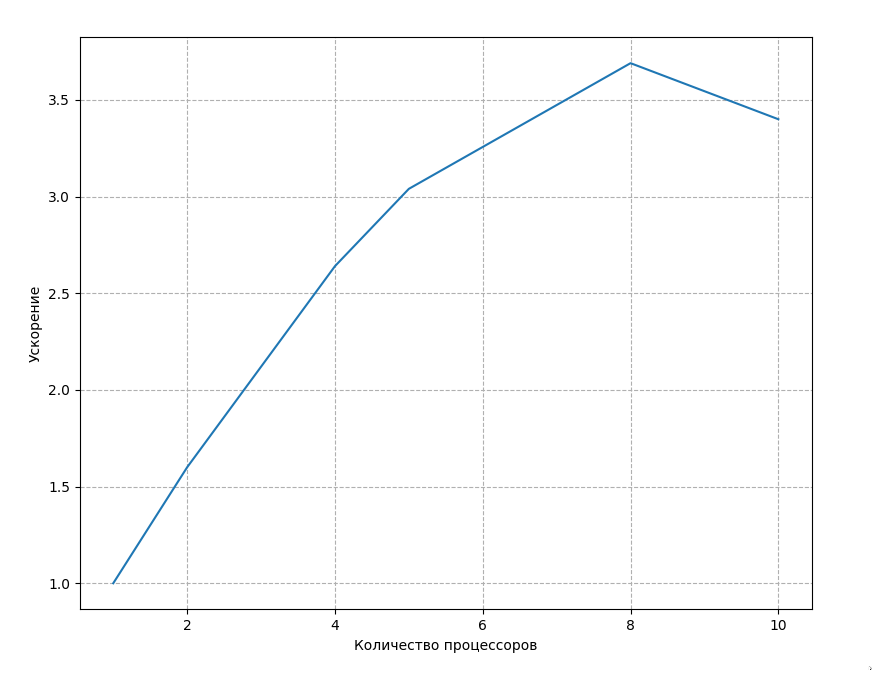
\includegraphics[width=\textwidth]{img/fst.png}
		\caption{ Зависимость значения ускорения от количества используемых процессоров (размер матрицы 800) }
		\label{img:first}
\end{figure}
	
Из представленного графика видно, что пик ускорения достигается при количестве процессоров, равному 8.

На графике \ref{img:second} представлена зависимость значения ускорения от количества используемых процессоров при размерах матрицы 1600.

\begin{figure}[H]
	\centering
	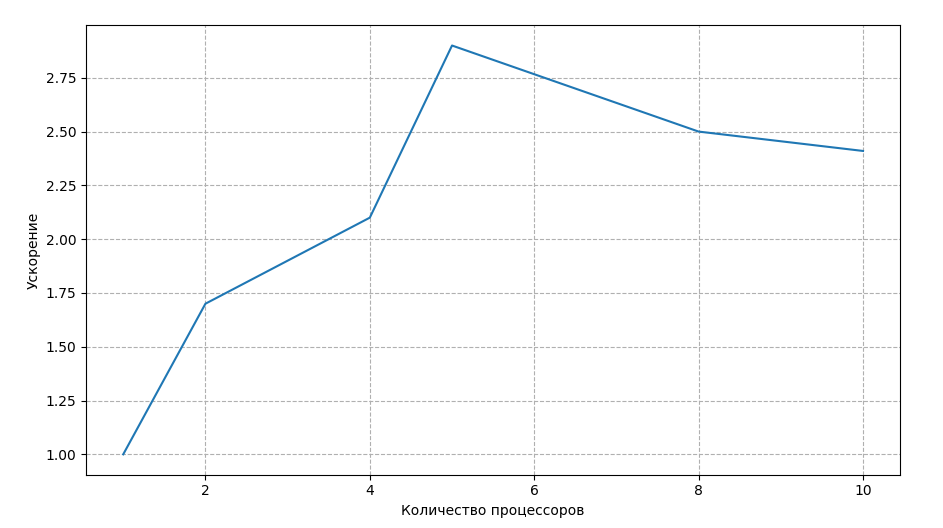
\includegraphics[width=\textwidth]{img/snd.png}
	\caption{ Зависимость значения ускорения от количества используемых процессоров (размер матрицы 1600)}
	\label{img:second}
\end{figure}

Из представленного графика видно, что пик ускорения достигается при количестве процессоров, равному 5.
	
\end{document}
